\section{Einleitung (Alle)}
Diese Arbeit beantwortet, ob neuronale Netze (NNs) in der Softwaretechnik (SWT) eingesetzt werden können und wo die Grenzen der Anwendungen liegen. Die Arbeit ist keine Umfrage, ob NNs in der Realität eingesetzt werden. Vielmehr werden drei Themengebiete vorgestellt, in denen Forscher NNs testeten und einsetzten. Die Auswahl wurde aufgrund von persönlichen Interessen und vorherrschender Brisanz getroffen. Unser Ziel war es, anhand der Themengebiete und konkreter Beispiele herauszufinden, ob und wie NNs in der SWT eingesetzt werden können, welche Probleme sie lösen und an welche Grenzen sie stoßen.
KNNs basieren auf der Funktion des biologischen Nervensystems. Informationen werden, wie bei einem menschlichen Gehirn auch, durch eine Vielzahl miteinander verknüpfter parallel laufender Neuronen  verarbeitet. Die daraus entstehenden Systeme trainieren sich teilweise selbst, um schnellere Entscheidungen treffen und Fehler vermeiden zu können \cite{technology}. 
NNs lassen sich in Kategorien unterteilen. Bekannte sind convolutional neural networks (CNNs), deep neural networks (DNNs), Residual neural networks (Resnets) und multilayer perception (MLP)-NNs. In dieser Arbeit wird näher auf CNNs und Resnets eingegangen. CNNs werden im Kapitel Spracherkennung näher erläutert, da die aufgeführten Beispiele auf CNNs bevorzugt eingehen. Resnets gehören zur Kategorie der DNNs. Jeder Layer des Resnets stellt ein sogenanntes Res dar und besitzt mehrere trainierbare Neuronen. Neuronen sind in Bezug auf KNNs Leiter und Überträger von Daten und Werten. Das Besondere ist der Dropout, welcher durch zufälliges Ausschalten von Neuronen Überanpassungen vermeidet \cite{residualnn}. Mehrschichtige neuronale Netze (Multilayer perceptrons) benutzen u.a. Back propagation, um Parameter für künstliche neuronale Netze zu trainieren. Back propagation dient dem Trainieren von Layern, genauer dessen Neuronen, um auf entstandene Fehler aufmerksam zu machen, welche rückwärts durch das NN gegeben werden, um die sogenannten shared weights neu auszurichten \cite{usingcnn}.\\

\section{Neuronale Netzwerke}
NNs werden verwendet, um unübersichtliche und komplizierte Probleme lösen. NNs bestehen aus Knotenelementen, den sog. Neuronen. Mehrere Neuronen bilden einen Layer. Bei herkömmlichen NNs wird zwischen drei Layer-Arten unterschieden, den Inputlayer, Hiddenlayer und Outputlayer. Inputlayer und Outputlayer sind in einem NN genau ein Mal vorhanden und dienen der Ein- und Ausgabe des NN. Zwischen diesen Schichten befinden sich beliebig viele Hiddenlayer. Jedes Neuron besitzt eine Verbindung zu allen Neuron der Folgenden Schicht. Von der jeweils oberen Schicht werden über diese Verbindungen Signale an die darunterliegende Schicht weitergeleitet. Eine Aktivierungsfunktion entscheidet in jedem Neuron, ob die eingetroffenen Signale für eine Weiterleitung ausreichen. Auf den Verbindungen liegen unterschiedliche Gewichtungen, die die Intensität eines Signals beeinflussen. Beim Training des NN werden die Gewichtungen angepasst.
Es gibt zwei grundsätzliche Trainingsansätze. Das supervised learning setzt einen Datensatz mit erwarteten Ergebnissen voraus. Nach Verarbeitung der Daten werden die Gewichte des NN anhand der Erwartungswerte angepasst. Ansätze für unsupervsed learning kommen auch ohne gekennzeichnete Daten aus, sind aber derzeit noch nicht einsatzfähig. NN können durch ihre trainierbarkeit komplexe Sachverhalte verarbeiten und bieten einen Lösungsansatz für zuvor unlösbare Probleme~\cite{Maind2014}\\
\vspace{6.0cm}
\begin{figure}[h]
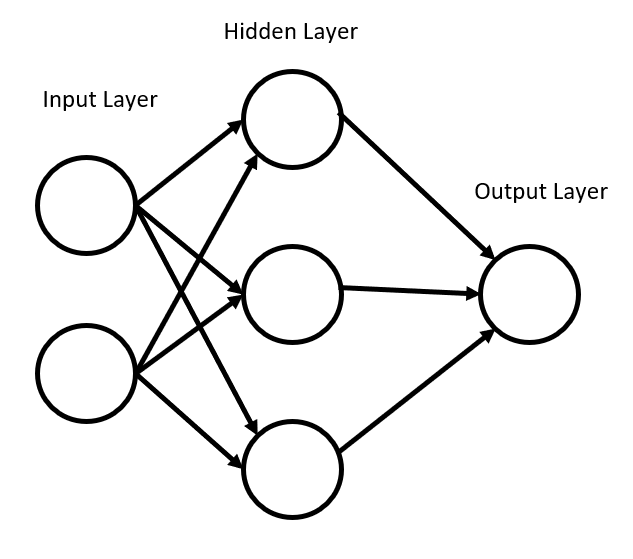
\includegraphics[width=\linewidth, height=6cm]{Bilder/NN/NeuralNetwork.png}
\caption{CNN-Architektur vgl. \cite{Maind2014}}
\end{figure}
\\


\\
\vspace{6.0cm}
\begin{figure}[h]
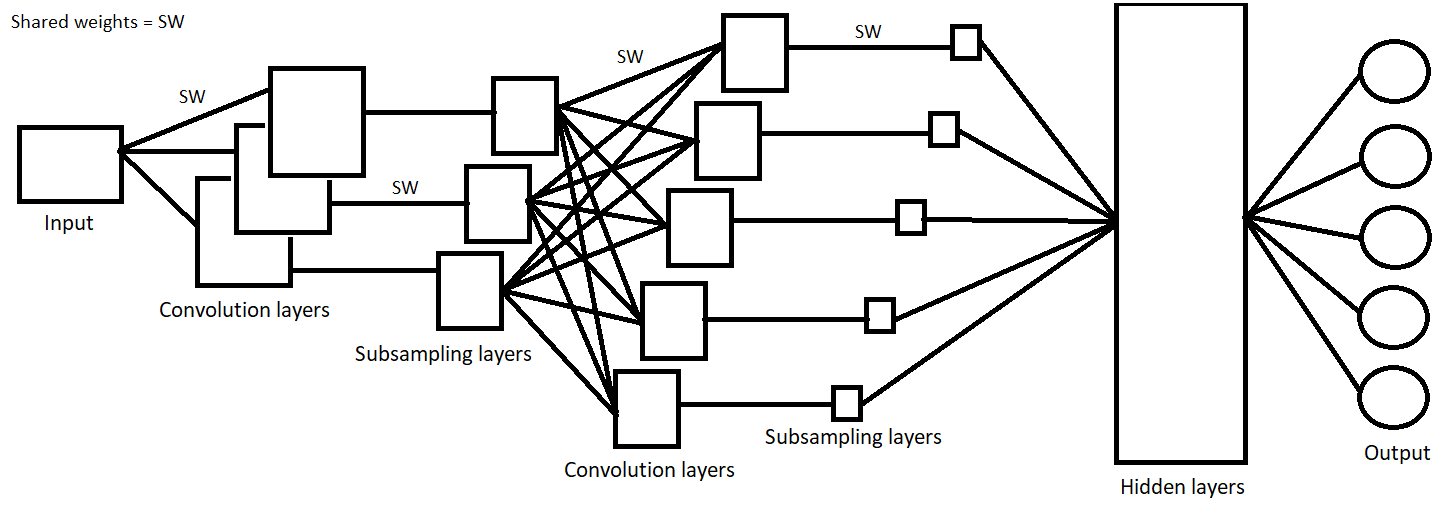
\includegraphics[width=\linewidth, height=6cm]{Bilder/CNN/CNNArchitektur.png}
\caption{CNN-Architektur vgl. \cite{noisycnn}}
\end{figure}
\\
Das Hidden Markov Model (HMM) ist bekannt für seinen Nutzen im Bereich der speech recognition \cite{residualnn}. HMM ist in der Lage Wörter zu modellieren, welche daraufhin einem bestimmten Kontext zugeordnet werden können. Der HMM-Algorithmus gehört zu den unsupervised learning techniques, da er Parameter unkontrolliert schätzt ohne zusätzliche Kennzeichnungen durch Menschen \cite{hmm}. Ein MLP-NN weißt während des Trainings jedem Neuron eine Gewichtung zu, um den Einfluss zwischen Input und Output zu maximieren \cite{Khalifelu2012}. Radial Basis Function-NNs (RBF) werden in den Gebieten der pattern recognition und Funktionsapproximation eingesetzt. In Kapitel \ref{Mustererkennung} wird die Disziplin Mustererkennung und dazugehörige Verfahren und Möglichkeiten näher beschrieben. Anschließend wird in Kapitel \ref{KostenAufwand} der Einsatz von NNs im Gebiet Kosten- und Aufwandsschätzung erläutert und damit verbundene Methoden und Praktiken aufgezeigt. Kapitel \ref{SQ} befasst sich mit NNs im Bereich Qualitätsmanagement und gibt einen Einblick auf verwendete Mittel und Vorgehensweisen, welche in dem genannten Bereich notwendig und nützlich sind. Letztendlich folgt ein Fazit, welches die Ergebnisse aus allen Kapiteln vereint, vergleicht und bewertet.

\vspace{3.0cm}